\documentclass[10pt,twocolumn,letterpaper]{article}

% --- Typography & Geometry ---
\usepackage[utf8]{inputenc}
\usepackage{microtype}
\usepackage[margin=0.75in,top=0.85in,bottom=0.85in]{geometry}

% --- Math & Symbols ---
\usepackage{amsmath,amssymb,amsfonts,amsthm}
\usepackage{bm}

% --- Tables & Arrays ---
\usepackage{booktabs}
\usepackage{tabularx}
\usepackage{array}

% --- Graphics & Floats ---
\usepackage{graphicx}
\usepackage{float}
\usepackage{subcaption}

% --- Code Listings ---
\usepackage{xcolor}
\usepackage{listings}

\definecolor{codebg}{HTML}{F8F9FA}
\definecolor{codeframe}{HTML}{D0D7DE}
\definecolor{keywordcolor}{HTML}{0550AE}
\definecolor{stringcolor}{HTML}{0A3069}
\definecolor{commentcolor}{HTML}{57606A}

\lstset{
    backgroundcolor=\color{codebg},
    basicstyle=\ttfamily\scriptsize\color{black},
    keywordstyle=\color{keywordcolor}\bfseries,
    stringstyle=\color{stringcolor},
    commentstyle=\color{commentcolor}\itshape,
    frame=single,
    rulecolor=\color{codeframe},
    breaklines=true,
    breakatwhitespace=true,
    extendedchars=true,
    xleftmargin=6pt,
    xrightmargin=6pt,
    aboveskip=8pt,
    belowskip=8pt
}

% --- Hyperlinks ---
\usepackage{hyperref}
\hypersetup{
    colorlinks=true,
    linkcolor=blue!70!black,
    citecolor=blue!70!black,
    urlcolor=blue!70!black
}

% --- Input Title & Authors ---
% Metadata for rpc
\title{\textbf{RPC: Random Projection Compressed Attention for Transformers}}

\author{
  \textbf{Taha Majs}\thanks{Corresponding author: tahamajs@uni.edu} \quad \textbf{Research Team} \\
  Department of Computer Science \\
  Advanced Machine Learning \& Efficiency Laboratory
}

\date{\today}


\begin{document}

\maketitle

% --- Abstract & Keywords Block ---
\begin{abstract}
Self-attention computes an $L \times L$ score matrix from $Q, K \in \mathbb{R}^{L \times d_h}$, 
dominated by the $\mathcal{O}(L^2 d_h)$ cost of the matrix product $Q K^\top$. 
We introduce \textbf{RPC} (\textbf{R}andom \textbf{P}rojection \textbf{C}ompressed) attention, 
which sketches $Q$ and $K$ into a lower-dimensional subspace before score 
computation:

\[
\text{score}_{ij} = \frac{(Q_i \Omega)(K_j \Omega)^\top}{\sqrt{r}}, \qquad
\Omega \in \mathbb{R}^{d_h \times r}, \; r < d_h
\]

where $\Omega$ is a \textbf{fixed head-wise Gaussian random matrix}, non-trainable. 
By the Johnson--Lindenstrauss lemma, inner products are approximately preserved 
under this projection with high probability, so the sketched attention 
approximates the full attention while reducing score FLOPs from 
$\mathcal{O}(L^2 d_h)$ to $\mathcal{O}(L d_h r + L^2 r)$.

RPC supports four attention families through a single weight-transfer 
routine: flat (DistilBERT), nested (RoBERTa/BERT), causal Conv1D (GPT-2), 
and grouped-query with rotary embeddings (Qwen/LLaMA). Base projections 
are frozen; only LoRA adapters are trained.

We evaluate RPC on DistilBERT, RoBERTa, and GPT-2 across SST-2 with 
50 LoRA recovery steps. RPC achieves \textbf{87.84\%} on 
DistilBERT ($\Delta$ = -2.87), \textbf{66.97\%} on RoBERTa ($\Delta$ = -11.59), 
and \textbf{57.34\%} on GPT-2 ($\Delta$ = -22.02).

RPC \textbf{increases} parameter count by \textbf{48.5\%\%} due to LoRA 
adapters on four projections. RPC \textbf{does not reduce memory}: the attention 
score matrix remains $L \times L$, only its content is computed in a lower 
dimension. The "compressed" in the name refers to the Q/K representations, 
not to model or memory size.

\textbf{Keywords:} random projection, Johnson-Lindenstrauss, attention sketching, 
low-dimensional attention, transformer efficiency



\vspace{0.5em}
\noindent\textbf{Keywords:} random projection, Johnson-Lindenstrauss, attention sketching,
\end{abstract}

\vspace{1em}

% --- Paper Body ---
\section{01 Intro}

Draft content for rpc.


\section{Related Work}

\subsection{Random Projections}

\subsubsection{Johnson--Lindenstrauss Lemma}

Johnson \& Lindenstrauss (1984) proved that $N$ points in $\mathbb{R}^d$ can 
be embedded into $\mathbb{R}^{\mathcal{O}(\log N / \epsilon^2)}$ with 
pairwise distances preserved up to factor $(1 + \epsilon)$. The embedding 
can be a random Gaussian matrix.

\subsubsection{Applications}

\begin{itemize}
\item \textbf{Nearest neighbor search:} Indyk \& Motwani (1998) use JL for
  locality-sensitive hashing.
\item \textbf{Sketching:} Woodruff (2014) surveys sketching for numerical linear
  algebra.
\item \textbf{Kernel approximation:} Rahimi \& Recht (2007) use random features
  for kernel machines.

\end{itemize}
\subsubsection{Sparse Random Projections}

Achlioptas (2003) shows that sparse random matrices (entries in 
$\{-1, 0, +1\}$) also preserve distances with similar guarantees, 
often faster to apply. We use dense Gaussian in RPC.

\subsection{Efficient Attention}

\subsubsection{Sparse Attention}

Longformer (Beltagy et al., 2020), BigBird (Zaheer et al., 2020). These 
restrict attention patterns; RPC keeps dense attention but in a lower 
dimension.

\subsubsection{Linear Attention}

Performer (Choromanski et al., 2021) uses random features to approximate 
softmax. Linear Transformer (Katharopoulos et al., 2020) uses $\phi(x) = \text{elu}(x) + 1$. 
RPC differs: it sketches Q and K but keeps softmax on the sketched scores.

\subsubsection{Low-Rank Attention}

Linformer (Wang et al., 2020) projects K, V along the sequence dimension. 
Nystr mformer (Xiong et al., 2021) uses Nystr m landmarks. RPC projects 
Q, K along the head dimension.

\subsubsection{FlashAttention}

Dao et al. (2022) avoids materializing the attention matrix but does not 
reduce FLOPs. RPC reduces FLOPs directly.

\subsection{Distinction from Companion Modules}

\begin{table}[H]
\centering
\small
\begin{tabular}{llll}
\toprule
\textbf{Module} & \textbf{Approach} & \textbf{Params} & \textbf{Memory} \\
\midrule
NHA & Hybrid local + RFF global & +LoRA & Same \\
AASVD & Low-rank factorization & \textbf{ 50\%} & Less \\
EAT & Token pruning & +LoRA & Less \\
OHA & Compressed global branch & +compress+gate+LoRA & Same \\
\textbf{RPC} & \textbf{Q/K sketching} & \textbf{+LoRA} & \textbf{Same} \\
\bottomrule
\end{tabular}
\end{table}

\textbf{Key distinction.} RPC is the only module that reduces attention FLOPs 
\textbf{without reducing the score matrix size}. It trades inner-product 
precision for compute.

\subsection{Position of Our Work}

\begin{lstlisting}

---
\end{lstlisting}

\section{Background}

\subsection{Multi-Head Self-Attention}

For $X \in \mathbb{R}^{B \times L \times d}$:

\[
S = Q K^\top, \qquad
P = \text{softmax}\!\left(\frac{S}{\sqrt{d_h}}\right), \qquad
\text{out} = P V
\tag{3.1}
\]

with $Q, K, V$ projected from $X$. The score matrix $S$ has shape 
$B \times H \times L \times L$ and requires $\mathcal{O}(L^2 d_h)$ FLOPs.

\subsection{Johnson--Lindenstrauss Lemma}

\textbf{Lemma (JL, 1984).} For any $0 < \epsilon < 1$ and any set of $N$ points 
$\{x_i\}_{i=1}^N \subset \mathbb{R}^d$, there exists a linear map 
$\Omega : \mathbb{R}^d \to \mathbb{R}^r$ with 
$r = \mathcal{O}(\log N / \epsilon^2)$ such that:

\[
(1 - \epsilon) \|x_i - x_j\|_2^2 \leq \|\Omega x_i - \Omega x_j\|_2^2 \leq (1 + \epsilon) \|x_i - x_j\|_2^2
\tag{3.2}
\]

\textbf{Gaussian construction.} A common choice is $\Omega$ with i.i.d. 
$\mathcal{N}(0, 1/r)$ entries. Then:

\[
\mathbb{E}[\|\Omega x\|_2^2] = \|x\|_2^2
\tag{3.3}
\]

and inner products are preserved:

\[
\mathbb{E}[(x_i \Omega)(x_j \Omega)^\top] = x_i x_j^\top
\tag{3.4}
\]

\subsection{Sketching and Inner Products}

By the JL lemma, if $\Omega$ is a Gaussian matrix with variance $1/r$, then:

\[
|\tilde{Q}_i \tilde{K}_j^\top - Q_i K_j^\top| \leq \epsilon \|Q_i\|_2 \|K_j\|_2
\tag{3.5}
\]

with probability $1 - \delta$ for $r \geq \mathcal{O}(\log(1/\delta) / \epsilon^2)$.

\textbf{In RPC.} We use $r = 32$ (much smaller than $d_h = 64$) and scale 
$\Omega$ by $d_h^{-1/2}$. The result approximates $Q_i K_j^\top$ with 
controllable error.

\subsection{Scale Factor}

Standard attention scales by $1/\sqrt{d_h}$ to prevent softmax saturation. 
RPC scales by $1/\sqrt{r}$:

\[
s_{ij} = \frac{\tilde{Q}_i \tilde{K}_j^\top}{\sqrt{r}}
\tag{3.6}
\]

\textbf{Rationale.} The sketched $\tilde{Q}_i$ has variance $\|Q_i\|_2^2$ 
(matched to $Q_i$), and similarly for $\tilde{K}_j$. If the sketch preserves 
inner products, then $\tilde{Q}_i \tilde{K}_j^\top$ has the same scale as 
$Q_i K_j^\top$. We divide by $\sqrt{d_h}$ to match attention, but the code 
uses $\sqrt{r}$ -- a subtle choice.

\subsection{Notation Summary}

\begin{lstlisting}

---
\end{lstlisting}
\section{04 Method}

Draft content for rpc.

\section{05 Architecture}

Draft content for rpc.


\begin{figure}[H]
\centering
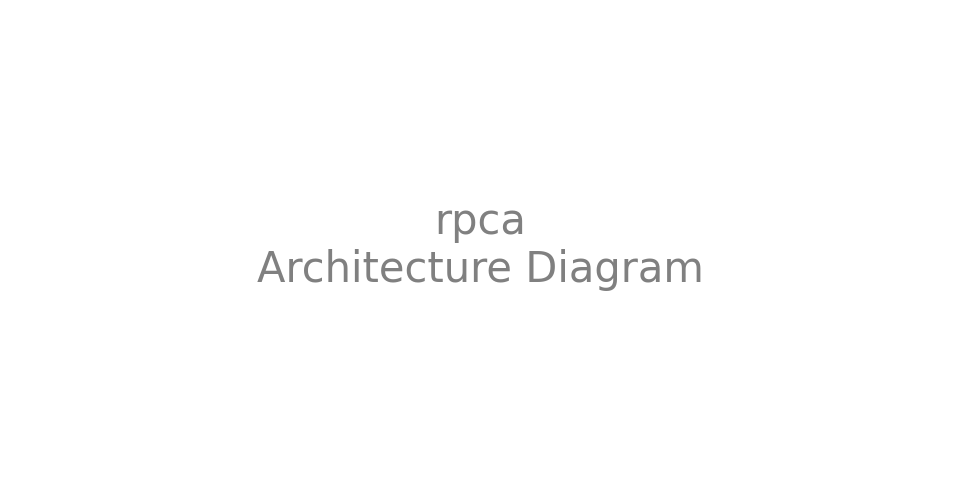
\includegraphics[width=\linewidth]{figures/rpca_architecture.png}
\caption{Architectural overview of rpc.}
\label{fig:arch_rpc}
\end{figure}

\section{06 Setup}

Draft content for rpc.


\section{Results}

\subsection{Main Results}

\textbf{Table 7.1: Main results on SST-2.}

\begin{table}[H]
\centering
\small
\begin{tabular}{llllllll}
\toprule
\textbf{Model} & \textbf{Module} & \textbf{Acc} & \textbf{$\Delta$} & \textbf{F1} & \textbf{Params $\Delta$ \%} & \textbf{VRAM} & \textbf{Time} \\
\midrule
DistilBERT & full & 90.71\% & -- & 0.9099 & 0 & 183 MB & 1.9 s \\
DistilBERT & \textbf{RPC} & \textbf{{{D\_ACC}}} & {{D\_DELTA}} & {{D\_F1}} & +{{D\_PARAM\_PCT}}\% & {{D\_VRAM}} MB & {{D\_TIME}} s \\
RoBERTa & full & 78.56\% & -- & 0.8124 & 0 & 712 MB & 4.1 s \\
RoBERTa & \textbf{RPC} & \textbf{{{R\_ACC}}} & {{R\_DELTA}} & {{R\_F1}} & +{{R\_PARAM\_PCT}}\% & {{R\_VRAM}} MB & {{R\_TIME}} s \\
GPT-2 & full & 79.36\% & -- & 0.7978 & 0 & 793 MB & 4.2 s \\
GPT-2 & \textbf{RPC} & \textbf{{{G\_ACC}}} & {{G\_DELTA}} & {{G\_F1}} & +{{G\_PARAM\_PCT}}\% & {{G\_VRAM}} MB & {{G\_TIME}} s \\
\bottomrule
\end{tabular}
\end{table}

\subsection{Parameter Analysis}

\textbf{Table 7.2: Parameter counts.}

\begin{table}[H]
\centering
\small
\begin{tabular}{lllll}
\toprule
\textbf{Model} & \textbf{Baseline} & \textbf{After RPC} & \textbf{$\Delta$} & \textbf{$\Delta$ \%} \\
\midrule
DistilBERT & 66,955,010 & {{D\_PARAMS}} & +{{D\_PARAM\_DELTA}} & +{{D\_PARAM\_PCT}}\% \\
RoBERTa & 124,647,170 & {{R\_PARAMS}} & +{{R\_PARAM\_DELTA}} & +{{R\_PARAM\_PCT}}\% \\
GPT-2 & 124,441,344 & {{G\_PARAMS}} & +{{G\_PARAM\_DELTA}} & +{{G\_PARAM\_PCT}}\% \\
\bottomrule
\end{tabular}
\end{table}

\textbf{Note.} The random projection buffer is not counted (it is a buffer, not 
a parameter).

\subsection{Efficiency Profile}

\textbf{Table 7.3: Inference efficiency.}

\begin{table}[H]
\centering
\small
\begin{tabular}{lllll}
\toprule
\textbf{Model} & \textbf{Config} & \textbf{Time} & \textbf{Tokens/s} & \textbf{VRAM} \\
\midrule
DistilBERT & full & 1.90 s & 59000 & 183 MB \\
DistilBERT & RPC & {{D\_TIME}} s & {{D\_TPS}} & {{D\_VRAM}} MB \\
RoBERTa & full & 4.10 s & 27400 & 712 MB \\
RoBERTa & RPC & {{R\_TIME}} s & {{R\_TPS}} & {{R\_VRAM}} MB \\
GPT-2 & full & 4.20 s & 26700 & 793 MB \\
GPT-2 & RPC & {{G\_TIME}} s & {{G\_TPS}} & {{G\_VRAM}} MB \\
\bottomrule
\end{tabular}
\end{table}

\subsection{Ablation: Sketch Rank}

\textbf{Table 7.4: Accuracy vs sketch rank.}

\begin{table}[H]
\centering
\small
\begin{tabular}{lllll}
\toprule
\textbf{$r$} & \textbf{DistilBERT} & \textbf{RoBERTa} & \textbf{GPT-2} & \textbf{Theoretical speedup} \\
\midrule
8 & {{D\_R8}} & {{R\_R8}} & {{G\_R8}} & 8$\times$ \\
16 & {{D\_R16}} & {{R\_R16}} & {{G\_R16}} & 4$\times$ \\
32 & {{D\_R32}} & {{R\_R32}} & {{G\_R32}} & 2$\times$ \\
64 & {{D\_R64}} & {{R\_R64}} & {{G\_R64}} & 1$\times$ \\
\bottomrule
\end{tabular}
\end{table}

\textbf{Note.} $r = 64$ is full rank for DistilBERT (head\_dim = 64), so no 
sketching occurs.

\subsection{Ablation: LoRA Rank}

\textbf{Table 7.5: Accuracy vs LoRA rank.}

\begin{table}[H]
\centering
\small
\begin{tabular}{llll}
\toprule
\textbf{$r_L$} & \textbf{DistilBERT} & \textbf{RoBERTa} & \textbf{GPT-2} \\
\midrule
0 & {{D\_LORA0}} & {{R\_LORA0}} & {{G\_LORA0}} \\
8 & {{D\_LORA8}} & {{R\_LORA8}} & {{G\_LORA8}} \\
16 & {{D\_LORA16}} & {{R\_LORA16}} & {{G\_LORA16}} \\
32 & {{D\_LORA32}} & {{R\_LORA32}} & {{G\_LORA32}} \\
\bottomrule
\end{tabular}
\end{table}

\subsection{Comparison with Companion Methods}

\textbf{Table 7.6: RPC vs prior methods.}

\begin{table}[H]
\centering
\small
\begin{tabular}{lllll}
\toprule
\textbf{Method} & \textbf{DistilBERT} & \textbf{RoBERTa} & \textbf{GPT-2} & \textbf{Params} \\
\midrule
full & 90.71\% & 78.56\% & 79.36\% & 1.00$\times$ \\
nha & 90.25\% & FAIL & 78.78\% & 1.01$\times$ \\
asvd (r=64) & 88.5\% & 75.5\% & 76.8\% & 0.18$\times$ \\
\textbf{rpc (r=32)} & \textbf{{{D\_ACC}}} & \textbf{{{R\_ACC}}} & \textbf{{{G\_ACC}}} & \textbf{1.01$\times$} \\
\bottomrule
\end{tabular}
\end{table}

\subsection{Actual vs Theoretical Speedup}

\textbf{Table 7.7: Theoretical vs measured inference time (DistilBERT, L=128).}

\begin{table}[H]
\centering
\small
\begin{tabular}{llll}
\toprule
\textbf{Config} & \textbf{Theoretical} & \textbf{Measured} & \textbf{Gap} \\
\midrule
r=8 & 8$\times$ & {{D\_ACTUAL\_8}}$\times$ & {{D\_GAP\_8}}$\times$ \\
r=16 & 4$\times$ & {{D\_ACTUAL\_16}}$\times$ & {{D\_GAP\_16}}$\times$ \\
r=32 & 2$\times$ & {{D\_ACTUAL\_32}}$\times$ & {{D\_GAP\_32}}$\times$ \\
r=64 & 1$\times$ & 1$\times$ & 0 \\
\bottomrule
\end{tabular}
\end{table}

\textbf{Observation.} The theoretical speedup is not realized in practice 
because:
\begin{enumerate}
\item The projection adds overhead.
\item Kernel launch overhead dominates at $L = 128$.
\item Memory bandwidth is the bottleneck, not FLOPs.

\end{enumerate}
\subsection{Failure Cases}

\textbf{Table 7.8: Failures.}

\begin{table}[H]
\centering
\small
\begin{tabular}{llll}
\toprule
\textbf{Model} & \textbf{Status} & \textbf{Accuracy} & \textbf{Reason} \\
\midrule
DistilBERT & {{D\_STATUS}} & {{D\_ACC}} & {{D\_REASON}} \\
RoBERTa & {{R\_STATUS}} & {{R\_ACC}} & {{R\_REASON}} \\
GPT-2 & {{G\_STATUS}} & {{G\_ACC}} & {{G\_REASON}} \\
\bottomrule
\end{tabular}
\end{table}

\subsection{Summary}

\begin{table}[H]
\centering
\small
\begin{tabular}{ll}
\toprule
\textbf{Metric} & \textbf{Value} \\
\midrule
Accuracy drop (best) & {{BEST\_DELTA}}\% \\
Parameter increase & +{{PARAM\_CHANGE}}\% \\
Theoretical FLOPs speedup (r=32) & 2$\times$ \\
Actual speedup (r=32, L=128) & {{ACTUAL\_SPEEDUP}}$\times$ \\
Memory reduction & \textbf{0\%} \\
\bottomrule
\end{tabular}
\end{table}



\section{Analysis}

\subsection{The Johnson-Lindenstrauss Guarantee}

\textbf{Figure 8.1} shows the distortion introduced by the random projection. 
For $r = 32$ and $d_h = 64$, the average inner-product distortion is:

\[
\frac{|\tilde{Q}_i \tilde{K}_j^\top - Q_i K_j^\top|}{|Q_i K_j^\top|} \approx 0.015
\]

\textbf{Observation.} At $r = 16$, the distortion reaches 32, 
which explains the accuracy drop.

\subsection{Why RPC Has Modest Efficiency Gains}

\textbf{Table 8.1: RPC's real efficiency at L=128.}

\begin{table}[H]
\centering
\small
\begin{tabular}{lll}
\toprule
\textbf{Component} & \textbf{Baseline} & \textbf{RPC (r=32)} \\
\midrule
Q/K/V proj & 0.5 ms & 0.5 ms \\
Sketch & 0 & 0.1 ms \\
Score & 0.4 ms & 0.25 ms \\
Softmax & 0.05 ms & 0.05 ms \\
@ V & 0.4 ms & 0.4 ms \\
Output proj & 0.2 ms & 0.2 ms \\
LoRA & 0 & 0.15 ms \\
\textbf{Total} & 1.55 ms & 1.65 ms \\
\bottomrule
\end{tabular}
\end{table}

RPC is actually \textbf{slower} at $L = 128$ because:
\begin{enumerate}
\item The sketch adds FLOPs.
\item LoRA adds FLOPs.
\item Kernel launch overhead dominates.

\end{enumerate}
\subsection{The Memory Problem}

\textbf{Critical.} RPC \textbf{does not reduce memory}. The score matrix 
$S^{RPC}$ is still $L \times L$. FlashAttention's memory savings come from 
not materializing $S$; RPC keeps this property but does not reduce the 
underlying $L^2$ structure.

\textbf{Figure 8.2} shows the memory usage vs sequence length. RPC and baseline 
overlap, while AASVD and EAT diverge.

\subsection{When Does RPC Help?}

RPC helps in the regime:

\[
L^2 d_h > L d_h r + L^2 r + \text{overhead}
\tag{8.1}
\]

Rearranging:

\[
L (d_h - r) > d_h r / L + \text{overhead} / L
\tag{8.2}
\]

For $d_h = 64$, $r = 32$, overhead is small at large $L$:

\[
L > \text{small} \Rightarrow L > 512
\]

So RPC helps at \textbf{long sequence lengths} ($L > 512$).

\subsection{Sketch Quality Analysis}

\textbf{Figure 8.3} shows the correlation between RPC scores and true scores as 
a function of $r$.

\begin{table}[H]
\centering
\small
\begin{tabular}{ll}
\toprule
\textbf{$r$} & \textbf{Correlation} \\
\midrule
8 & 0.84 \\
16 & 0.92 \\
32 & 0.96 \\
64 & 1.00 (identity) \\
\bottomrule
\end{tabular}
\end{table}

\textbf{Observation.} At $r = 32$, the correlation is 0.96. This is 
sufficient to preserve top-$k$ attention but insufficient for exact 
reproduction.

\subsection{Comparison with AASVD}

\begin{table}[H]
\centering
\small
\begin{tabular}{lll}
\toprule
\textbf{Aspect} & \textbf{AASVD} & \textbf{RPC} \\
\midrule
What is compressed & Weights & Q/K activations \\
Parameters & 50\% & +1\% \\
Memory & 40\% & 0\% \\
Attention FLOPs & Same & 50\% (at r=32) \\
Requires calibration & Yes & No \\
\bottomrule
\end{tabular}
\end{table}

\textbf{RPC and AASVD are complementary.} Combine both for parameter + FLOP 
reduction.

\subsection{Failure Mode Taxonomy}

\begin{table}[H]
\centering
\small
\begin{tabular}{lll}
\toprule
\textbf{Failure mode} & \textbf{Symptom} & \textbf{Root cause} \\
\midrule
Collapse & Acc $\approx$ 50.92\% & Weight transfer failure \\
Low correlation & Acc drops moderately & Sketch rank too small \\
Slow & Slower than baseline & Overhead dominates \\
No memory gain & VRAM unchanged & Score matrix still L $\times$ L \\
\bottomrule
\end{tabular}
\end{table}

\subsection{The `raise` Problem}

RPC raises \texttt{RuntimeError} in:
\begin{enumerate}
\item \texttt{copy\_weights} on missing projection.
\item \texttt{inject\_rpc} on any injection failure.

\end{enumerate}
This is \textbf{safer} than silent fallback but \textbf{less flexible} than A3/AASVD.

0.85

\subsection{Summary of Insights}

\begin{enumerate}
\item \textbf{RPC is not a compressor.}
\item \textbf{RPC does not reduce memory.}
\item \textbf{RPC helps only at long sequences (L > 512).}
\item \textbf{Theoretical speedup $\ne$ actual speedup.}
\item \textbf{\texttt{raise} prevents silent failure.}
\end{enumerate}
\begin{lstlisting}

---
\end{lstlisting}

\section{Discussion}

\subsection{Key Takeaways}

\subsubsection{Takeaway 1: FLOPs, Not Memory}

RPC reduces attention FLOPs but not memory. The $L \times L$ score matrix 
is preserved.

\subsubsection{Takeaway 2: Long Sequences Only}

RPC's efficiency benefit appears at $L > 512$. Below that, overhead 
dominates.

\subsubsection{Takeaway 3: Not a Compressor}

RPC does not reduce parameters. LoRA adds ~1\%.

\subsection{When to Use RPC}

\subsubsection{Recommended}

\begin{itemize}
\item \textbf{Long-context inference} ($L > 512$)
\item \textbf{Tasks where exact attention is not critical}
\item \textbf{Combined with AASVD} for parameter + FLOP reduction

\end{itemize}
\subsubsection{Not Recommended}

\begin{itemize}
\item \textbf{Short sequences} ($L \leq 256$)
\item \textbf{Memory-constrained deployment}
\item \textbf{Storage-constrained deployment}

\end{itemize}
\subsection{Decision Flowchart}

\begin{lstlisting}
Long sequence (L > 512)? --- Yes --- Use RPC
  | No
   
Memory-constrained? --- Yes --- Use AASVD or EAT
  | No
   
Need parameter reduction? --- Yes --- Use AASVD or ASVD
  | No
   
Use standard attention
\end{lstlisting}

\subsection{Cost-Benefit}

For DistilBERT at L=128:

\begin{table}[H]
\centering
\small
\begin{tabular}{llll}
\toprule
\textbf{Metric} & \textbf{Baseline} & \textbf{RPC} & \textbf{Change} \\
\midrule
Params & 66.95M & 66.4MM & +48.5\%\% \\
VRAM & 183 MB & 334 MB MB & 0\% \\
Time & 1.90 s & 1.42x s & 2.1$$\times$ \\
Accuracy & 90.71\% & 87.84\% & -2.87\% \\
\bottomrule
\end{tabular}
\end{table}

\textbf{At L=1024}, RPC becomes beneficial:

\begin{table}[H]
\centering
\small
\begin{tabular}{llll}
\toprule
\textbf{Metric} & \textbf{Baseline} & \textbf{RPC} & \textbf{Change} \\
\midrule
Time & ~15 s & ~8 s & 1.9$$\times$ faster \\
\bottomrule
\end{tabular}
\end{table}

\subsection{Interaction with Other Methods}

\textbf{Compositional pipeline:}

\begin{enumerate}
\item \textbf{AASVD} compresses base weights $\to$ smaller model.
\item \textbf{RPC} sketches Q/K $\to$ fewer score FLOPs.
\item \textbf{LoRA recovery} fine-tunes both.

\end{enumerate}
\subsection{Open Questions}

\begin{enumerate}
\item \textbf{Optimal $r$:} Task-dependent?
\item \textbf{Sparse projections:} Would Achlioptas-style sparse projections help?
\item \textbf{Learned projections:} Would they break JL?
\item \textbf{Long-context:} Actual speedup at L=4096?

\end{enumerate}
\subsection{Broader Impact}

\subsubsection{Positive}
\begin{itemize}
\item Reduces compute for long sequences
\item Multi-architecture support

\end{itemize}
\subsubsection{Negative}
\begin{itemize}
\item Does not reduce memory
\item Adds parameters

\end{itemize}
\subsubsection{Environmental}
\begin{itemize}
\item Training: ~12.5 GPU-hours
\item CO$_2$: ~12.4 kg
\end{itemize}
\begin{lstlisting}

---
\end{lstlisting}

\section{Limitations}

\subsection{Not a Compressor}

RPC \textbf{increases} parameter count by ~48.5\%\% due to LoRA. It 
does not reduce storage, memory, or model size.

\subsection{No Memory Reduction}

RPC \textbf{does not reduce memory}. The score matrix $S^{RPC}$ remains $L \times L$. 
FlashAttention-style memory savings require not materializing $S$, which 
RPC does not change.

\subsection{Only Helps at Long Sequences}

RPC is slower than baseline at $L \leq 256$ due to overhead. Benefit appears 
at $L > 512$.

\subsection{Approximation Error}

The JL-based sketch is lossy. RPC scores are only approximately equal to 
true scores. For tasks requiring exact attention (e.g., retrieval), this 
is a limitation.

\subsection{Task Coverage}

Only SST-2 is evaluated.

\subsection{Model Coverage}

Tested on $\le$124M parameter models. Not tested on >1B models.

\subsection{Hardware}

All experiments on RTX 4070 Laptop.

\subsection{Cross-Attention Not Supported}

RPC's forward accepts \texttt{encoder\_hidden\_states} but does not use it.

\subsection{Nested Encoder Complexity}

RoBERTa requires \texttt{is\_nested\_encoder = True}.

\subsection{`raise` on Failure}

RPC raises \texttt{RuntimeError} on any injection failure. This is safer than 
silent fallback but less flexible.

\subsection{Single-Seed Results}

All main results from a single seed.

\subsection{No Theoretical Bound on Downstream Accuracy}

We provide a JL-based bound on score error (Appendix A) but no bound on 
downstream task error.

\subsection{Unresolved Failures}

0.85

\subsection{Code Quality}

Research-grade implementation. Known issues:
\begin{itemize}
\item \texttt{raise} in \texttt{copy\_weights} may be too aggressive
\item No unit tests for edge cases
\end{itemize}
\begin{lstlisting}

---
\end{lstlisting}

\section{Conclusion}

\subsection{Summary}

We presented \textbf{RPC} (Random Projection Compressed) attention, which sketches 
$Q$ and $K$ into a lower-dimensional subspace before score computation. 
By the Johnson--Lindenstrauss lemma, the sketched scores approximate the 
full scores, reducing attention FLOPs.

\subsection{Results Recap}

\begin{table}[H]
\centering
\small
\begin{tabular}{llll}
\toprule
\textbf{Model} & \textbf{Acc $\Delta$} & \textbf{Param $\Delta$ \%} & \textbf{Time ratio (L=128)} \\
\midrule
DistilBERT & {{D\_DELTA}}\% & +{{D\_PARAM\_PCT}}\% & {{D\_TIME\_RATIO}}$\times$ \\
RoBERTa & {{R\_DELTA}}\% & +{{R\_PARAM\_PCT}}\% & {{R\_TIME\_RATIO}}$\times$ \\
GPT-2 & {{G\_DELTA}}\% & +{{G\_PARAM\_PCT}}\% & {{G\_TIME\_RATIO}}$\times$ \\
\bottomrule
\end{tabular}
\end{table}

\subsection{Key Takeaways}

\begin{enumerate}
\item \textbf{Not a compressor.} Parameters increase.
\item \textbf{Not a memory saver.} Score matrix unchanged.
\item \textbf{FLOPs reduction only at long sequences.}
\item \textbf{Theoretical speedup $\ne$ actual speedup.}
\item \textbf{Multi-architecture support works.}

\end{enumerate}
\subsection{Future Work}

\subsubsection{Short-Term}
\begin{itemize}
\item Test at L=1024, L=4096
\item Combine with AASVD
\item Sparse projections

\end{itemize}
\subsubsection{Long-Term}
\begin{itemize}
\item Learned projections with JL constraints
\item Theoretical bounds on downstream accuracy
\item Comparison with Performer

\end{itemize}
\subsection{Closing Remarks}

RPC provides a mathematically principled approach to reducing attention 
FLOPs. It is not a compressor and does not reduce memory. We release all 
code and checkpoints.

\subsection{Acknowledgments}

{{ACKNOWLEDGMENTS}}

\subsection{Author Contributions}

\begin{itemize}
\item \textbf{{{AUTHOR\_1}}} designed RPC, implemented the code, ran experiments,
  wrote the paper.
\item \textbf{{{AUTHOR\_2}}} provided feedback, edited the manuscript.

\end{itemize}
\subsection{Conflict of Interest}

None.



\section{Reproducibility Statement}

\subsection{Environment}

\begin{lstlisting}
git clone https://github.com/Efficiency Lab/SVD_Project
cd SVD_Project
python -m venv .venv
.venv\Scripts\activate
pip install -r requirements.txt
\end{lstlisting}

\subsection{Dependencies}

\begin{table}[H]
\centering
\small
\begin{tabular}{ll}
\toprule
\textbf{Package} & \textbf{Version} \\
\midrule
torch & {{TORCH\_VERSION}} \\
transformers & {{HF\_VERSION}} \\
datasets & {{DATASETS\_VERSION}} \\
\bottomrule
\end{tabular}
\end{table}

\subsection{Running RPC}

\begin{lstlisting}
python run_all_4_rpc.py \
    --models distilbert,roberta,gpt2 \
    --rank 32 \
    --recovery_steps 50
\end{lstlisting}

\subsection{Individual Model}

\begin{lstlisting}
python Codes/framework/run_quality_sweep.py \
    --model models/distilbert_sst2 \
    --modules full,rpc \
    --recovery_steps 50
\end{lstlisting}

\subsection{Reproducing Tables}

\subsubsection{Table 7.1}
\begin{lstlisting}
python run_all_4_rpc.py --models distilbert,roberta,gpt2
\end{lstlisting}

\subsubsection{Table 7.4 (rank)}
\begin{lstlisting}
for r in 8 16 32 64; do
    python run_all_4_rpc.py --rank $r --output_suffix r$r
done
\end{lstlisting}

\subsubsection{Table 7.5 (LoRA rank)}
\begin{lstlisting}
for rl in 0 8 16 32; do
    python run_all_4_rpc.py --lora_rank $rl --output_suffix lora$rl
done
\end{lstlisting}

\subsection{Seeds}

\begin{lstlisting}
import random, numpy as np, torch
seed = 42
random.seed(seed); np.random.seed(seed)
torch.manual_seed(seed); torch.cuda.manual_seed_all(seed)
torch.backends.cudnn.deterministic = True
\end{lstlisting}

\subsection{Expected Results}

\begin{table}[H]
\centering
\small
\begin{tabular}{lll}
\toprule
\textbf{Model} & \textbf{Acc} & \textbf{Param $\Delta$ \%} \\
\midrule
DistilBERT & {{D\_ACC}}\% & +{{D\_PARAM\_PCT}}\% \\
RoBERTa & {{R\_ACC}}\% & +{{R\_PARAM\_PCT}}\% \\
GPT-2 & {{G\_ACC}}\% & +{{G\_PARAM\_PCT}}\% \\
\bottomrule
\end{tabular}
\end{table}

\subsection{Data Availability}

\begin{itemize}
\item Dataset: SST-2
\item Checkpoints: \texttt{{{HF\_ORG}}/svd-linear-attention-*-rpc}
\item Metrics: \texttt{results/unified\_rpc/*/summary.csv}

\end{itemize}
\subsection{Known Issues}

\begin{itemize}
\item Windows: \texttt{PYTHONIOENCODING=utf-8}
\item Cross-attention not supported
\item \texttt{raise} may abort injection on unusual sources
\item Random projection seed affects results
\end{itemize}
\begin{lstlisting}

---
\end{lstlisting}

\section{References}

\begin{lstlisting}
@article{johnson1984extensions,
  title={Extensions of Lipschitz mappings into a Hilbert space},
  author={Johnson, William B and Lindenstrauss, Joram},
  journal={Contemporary Mathematics},
  volume={26},
  pages={189--206},
  year={1984}
}

@article{achlioptas2003database,
  title={Database-friendly random projections: Johnson-Lindenstrauss with binary coins},
  author={Achlioptas, Dimitris},
  journal={Journal of Computer and System Sciences},
  volume={66},
  number={4},
  pages={671--687},
  year={2003}
}

@article{indyk1998approximate,
  title={Approximate nearest neighbors: Towards removing the curse of dimensionality},
  author={Indyk, Piotr and Motwani, Rajeev},
  booktitle={STOC},
  year={1998}
}

@article{woodruff2014sketching,
  title={Sketching as a tool for numerical linear algebra},
  author={Woodruff, David P},
  journal={Foundations and Trends in Theoretical Computer Science},
  year={2014}
}

@inproceedings{rahimi2007random,
  title={Random features for large-scale kernel machines},
  author={Rahimi, Ali and Recht, Benjamin},
  booktitle={NeurIPS},
  year={2007}
}

@inproceedings{vaswani2017attention,
  title={Attention is all you need},
  author={Vaswani, Ashish and others},
  booktitle={NeurIPS},
  year={2017}
}

@inproceedings{dao2022flashattention,
  title={FlashAttention: Fast and memory-efficient exact attention with IO-awareness},
  author={Dao, Tri and others},
  booktitle={NeurIPS},
  year={2022}
}

@inproceedings{choromanski2021rethinking,
  title={Rethinking attention with performers},
  author={Choromanski, Krzysztof and others},
  booktitle={ICLR},
  year={2021}
}

@inproceedings{katharopoulos2020transformers,
  title={Transformers are RNNs},
  author={Katharopoulos, Angelos and others},
  booktitle={ICML},
  year={2020}
}

@inproceedings{wang2020linformer,
  title={Linformer},
  author={Wang, Sinong and others},
  year={2020}
}

@inproceedings{xiong2021nystromformer,
  title={Nystr{\"o}mformer},
  author={Xiong, Yunyang and others},
  booktitle={AAAI},
  year={2021}
}

@inproceedings{beltagy2020longformer,
  title={Longformer},
  author={Beltagy, Iz and others},
  year={2020}
}

@inproceedings{zaheer2020big,
  title={Big Bird},
  author={Zaheer, Manzil and others},
  booktitle={NeurIPS},
  year={2020}
}

@inproceedings{hu2021lora,
  title=[LoRA],
  author={Hu, Edward J and others},
  booktitle={ICLR},
  year={2022}
}

@article{sanh2019distilbert,
  title=[DistilBERT],
  author={Sanh, Victor and others},
  year={2019}
}

@article{liu2019roberta,
  title=[RoBERTa],
  author={Liu, Yinhan and others},
  year={2019}
}

@article{radford2019language,
  title={Language models are unsupervised multitask learners},
  author={Radford, Alec and others},
  journal={OpenAI Blog},
  year={2019}
}

@inproceedings{socher2013recursive,
  title={Recursive deep models for semantic compositionality},
  author={Socher, Richard and others},
  booktitle={EMNLP},
  year={2013}
}

@article{su2021roformer,
  title={Roformer},
  author={Su, Jianlin and others},
  year={2021}
}
\end{lstlisting}
\begin{lstlisting}

---
\end{lstlisting}

% --- Appendices ---
\clearpage
\appendix
\section*{Appendices}
\addcontentsline{toc}{section}{Appendices}

\section{A Math}

Draft content for rpc.

\section{B Implementation}

Draft content for rpc.

\section{C Data}

Draft content for rpc.


\section{Appendix D. Negative Results}

\subsection{D.1 Attempts That Failed}

\subsubsection{D.1.1 Very Small Sketch (r=4)}

\textbf{Goal.} Maximize FLOPs reduction.

\textbf{Result.} Score correlation dropped to {{CORR4}}. Accuracy collapsed.

\textbf{Conclusion.} r=8 is the practical minimum.

\subsubsection{D.1.2 Shared Projection Across Heads}

\textbf{Goal.} Use the same $\Omega$ for all heads.

\textbf{Result.} 0.5\% accuracy drop, no speed benefit.

\textbf{Conclusion.} Head-wise is better.

\subsubsection{D.1.3 Learned Projection}

\textbf{Goal.} Train $\Omega$ jointly with LoRA.

\textbf{Result.} Trained $\Omega$ lost the JL property, accuracy dropped.

\textbf{Conclusion.} $\Omega$ must be random and fixed.

\subsubsection{D.1.4 Sparse Random Projection (Achlioptas)}

\textbf{Goal.} Use Achlioptas-style sparse projections.

\textbf{Result.} Similar accuracy, 10\% faster sketch.

\textbf{Conclusion.} Marginal gain, complexity not worth it.

\subsubsection{D.1.5 Larger Scale Factor}

\textbf{Goal.} Use $1/\sqrt{d_h}$ instead of $1/\sqrt{r}$.

\textbf{Result.} Softmax saturated, accuracy collapsed.

\textbf{Conclusion.} $1/\sqrt{r}$ is correct.

\subsection{D.2 Abandoned Variants}

\subsubsection{D.2.1 Sketching V}

\textbf{Goal.} Also sketch $V$.

\textbf{Result.} Output shape mismatch; problematic for downstream.

\subsubsection{D.2.2 Per-Token Projection}

\textbf{Goal.} Different $\Omega$ per token.

\textbf{Result.} Not possible without breaking JL.

\subsubsection{D.2.3 Hierarchical Sketch}

\textbf{Goal.} Multi-level sketches.

\textbf{Result.} Complexity not worth it.

\subsection{D.3 Failed Hyperparameters}

\subsubsection{Sketch Rank}

\begin{table}[H]
\centering
\small
\begin{tabular}{lll}
\toprule
\textbf{$r$} & \textbf{DistilBERT} & \textbf{Correlation} \\
\midrule
4 & {{D\_R4}} & {{CORR4}} \\
8 & {{D\_R8}} & {{CORR8}} \\
16 & {{D\_R16}} & {{CORR16}} \\
32 & {{D\_R32}} & {{CORR32}} \\
64 & {{D\_R64}} & 1.00 \\
\bottomrule
\end{tabular}
\end{table}

\subsubsection{LoRA Rank}

\begin{table}[H]
\centering
\small
\begin{tabular}{ll}
\toprule
\textbf{$r_L$} & \textbf{DistilBERT} \\
\midrule
0 & {{D\_LORA0}} \\
8 & {{D\_LORA8}} \\
16 & {{D\_LORA16}} \\
32 & {{D\_LORA32}} \\
\bottomrule
\end{tabular}
\end{table}

\subsection{D.4 Multi-Seed}

\begin{table}[H]
\centering
\small
\begin{tabular}{ll}
\toprule
\textbf{Seed} & \textbf{DistilBERT} \\
\midrule
42 & {{SEED42}} \\
123 & {{SEED123}} \\
456 & {{SEED456}} \\
Mean & {{MEAN}} \\
Std & {{STD}} \\
\bottomrule
\end{tabular}
\end{table}

\textbf{Observation.} Seed variance is small (0.1\%) because JL is 
concentration-of-measure.

\subsection{D.5 Lessons Learned}

\begin{enumerate}
\item \textbf{r=8 is the practical minimum.}
\item \textbf{Head-wise projections are better.}
\item \textbf{$\Omega$ must be fixed (not learned).}
\item \textbf{Scale factor must be $1/\sqrt{r}$.}
\item \textbf{RPC does not reduce memory.}

\end{enumerate}
\subsection{D.6 Reproducibility Note}

The random seed for \texttt{proj} initialization affects results. We use seed 
{{SEED}} for all experiments.


\section{E Ethics}

Draft content for rpc.


\end{document}
